%% \CharacterTable
%%  {Upper-case    \A\B\C\D\E\F\G\H\I\J\K\L\M\N\O\P\Q\R\S\T\U\V\W\X\Y\Z
%%   Lower-case    \a\b\c\d\e\f\g\h\i\j\k\l\m\n\o\p\q\r\s\t\u\v\w\x\y\z
%%   Digits        \0\1\2\3\4\5\6\7\8\9
%%   Exclamation   \!     Double quote  \"     Hash (number) \#
%%   Dollar        \$     Percent       \%     Ampersand     \&
%%   Acute accent  \'     Left paren    \(     Right paren   \)
%%   Asterisk      \*     Plus          \+     Comma         \,
%%   Minus         \-     Point         \.     Solidus       \/
%%   Colon         \:     Semicolon     \;     Less than     \<
%%   Equals        \=     Greater than  \>     Question mark \?
%%   Commercial at \@     Left bracket  \[     Backslash     \\
%%   Right bracket \]     Circumflex    \^     Underscore    \_
%%   Grave accent  \`     Left brace    \{     Vertical bar  \|
%%   Right brace   \}     Tilde         \~}
%\iffalse
%
% oinuit.dtx
% Copyright 2002 Apostolos Syropoulos
%
% This program may be distributed and/or modified under the
% conditions of the LaTeX Project Public License, either version 1.2
% of this license or (at your option) any later version.
% The latest version of this license is in
%   http://www.latex-project.org/lppl.txt
% and version 1.2 or later is part of all distributions of LaTeX 
% version 1999/12/01 or later.
%
% This program consists of the files oinuit.dtx and oinuit.ins
%
% Please report errors or suggestions for improvement to
%    
%    Apostolos Syropoulos
%    366, 28th October Str.
%    GR-671 00 Xanthi, GREECE
%    apostolo@ocean1.ee.duth.gr or apostolo@obelix.ee.duth.gr
%
%\fi
% \CheckSum{475}
% \iffalse This is a Metacomment
%
%<oinuit, >\ProvidesPackage{oinuit.sty}
%<LITenc, >\ProvidesFile{litenc.def}
%<LITcmr, >\ProvidesFile{litcmr.fd}
%<Hyphenation, >\message{2002/07/21 v1.0 Inuktitut hyphenation patterns}
%<Ninuit2uni, >%% Omega translation process Ninuit2uni
%<Qinuit2uni, >%% Omega translation process Qinuit2uni
%<inuitscii, >%% Omega translation process inuitscii
%
%<oinuit, >[2002/07/21 v1.0 Package `oinuit.sty']
%<LITenc, >[2002/07/21 v1.0 Local Inuktitut Encoding]
%<LITcmr, >[2002/07/21 v1.0 Inuktitut Font Definition]
%<Ninuit2uni, >%% 2002/07/21 v1.0 Inuktitut Latin transcription to Unicode,
%<Ninuit2uni, >%% follows the Anglican orthography.
%<Qinuit2uni, >%% 2002/07/21 v1.0 Inuktitut Latin transcription to Unicode,
%<Qinuit2uni, >%% follows the Catholic orthography.
%<inuitscii, >%% 2002/07/21 v1.0 Inuit ASCII to Unicode.
%
%    \begin{macrocode}
%<*driver>
\documentclass{ltxdoc}
\usepackage{url,graphicx}
\GetFileInfo{oinuit.drv}
\begin{document}
   \frenchspacing
   \DocInput{oinuit.dtx}
\end{document}
%</driver>
%    \end{macrocode}
% \fi
%
% \title{The \textit{oinuit} package}
% \author{Apostolos Syropoulos\\366, 28th October Str.\\
%         GR-671 00 Xanthi, HELLAS\\ 
%         Email:\texttt{apostolo@obelix.ee.duth.gr}\\ or \\
%         \hphantom{Email:}\texttt{apostolo@ocean1.ee.duth.gr}}
%         \date{2002/07/21}
% \maketitle
% 
%\MakeShortVerb{\|}
%\StopEventually{}
%
%  \section{Introduction}
%
% This $\Lambda$\footnote{$\Lambda$ is \LaTeX's nickname when used with the
% $\Omega$ typesetting engine.} package is part of a system that
% provides a rather complete solution to the problem of typesetting Inuktitut
% documents. The package is bundled with a PostScript version of the Nunacom 
% TrueType font developed by Nortext (\url{http://www.nortext.com}), which is 
% redistributed with permission from Nortext. In addition, there four $\Omega$
% virtual fonts, which define a Unicode encoded font that consists of the 
% English alphabet, the digits, some symbols and the Inuktitut syllabary.
%
% Inuktitut is the language of the Inuit (also known as Eskimos, but the term 
% is considered offensive by Inuit who live in Canada and Greenland). The 
% language is spoken in Greenland, Canada, Alaska, and the Chukotka Autonomous
% Okrug, which is located in the far northeast region of the Russian 
% Federation, by approximately 152,000 people. The Inuktitut syllabics are 
% used by Inuit who live in Canada, especially in the new Canadian territory 
% of Nunavut. This writing system was invented by Reverend James Evans, a 
% Wesleyan missionary. This system was based on earlier work on the Cree 
% language, which, in turn, was based on work on the Ojibway language.
% 
% The complete system consists of the following files:
% \begin{description}
% \item[\texttt{driver}]  produces a documentation driver file.
% \item[\texttt{oinuit.sty}]  the package itself.
% \item[\texttt{litenc.def}] font encoding definition file.
% \item[\texttt{litcmr.fd}]  font definition file.
% \item[\texttt{inuit.tex}]  Inuktitut hyphenation patterns.
% \item[\texttt{Ninuit2uni.otp}] an $\Omega$TP that transforms text written 
%      in the Inuktitut Latin transcription to Unicode that follows the 
%      Anglican orthography.
% \item[\texttt{Qinuit2uni.otp}]  an $\Omega$TP that transforms text written 
%      in the Inuktitut Latin transcription to Unicode that follows the 
%      Catholic orthography.
% \item[\texttt{inuitscii.otp}] an $\Omega$TP that transforms text written in 
%       a Inuit ASCII to Unicode. 
% \end{description}
% 
%  \section{The package `oinuit'}
%
% The package `oinuit' provides the basic user-interface for the typesetting
% of Inuktitut text with $\Lambda$. The package provides five options:
% \texttt{nunavut} (default option), \texttt{quebec}, \texttt{iscii},
% \texttt{utf8}, and \texttt{ucs2}, which should be used when users want to
% enter text using the Latin transcription of Inuktitut and the Anglican
% orthography, the Latin transcription of Inuktitut and the Catholic
% orthography, the Inuit ASCII (see Table~\ref{iscii}), the UTF-8 Unicode, 
% or the UCS-2 Unicode encoding, respectively.
% \begin{table}  
% \begin{center}
% 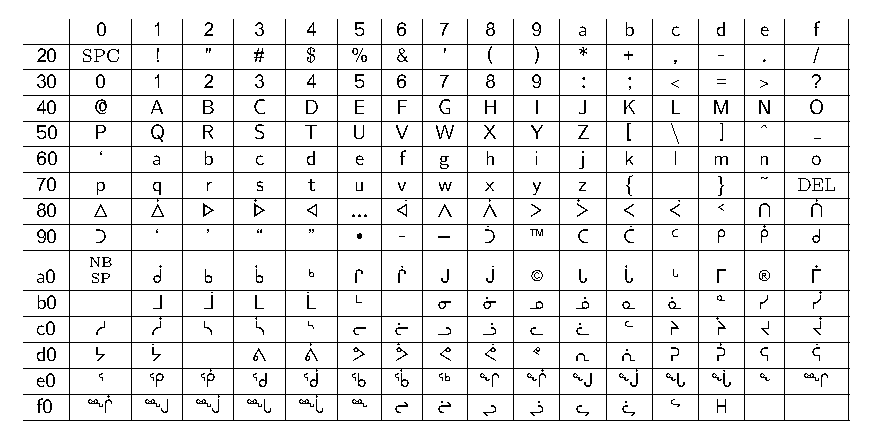
\includegraphics[scale=0.8]{Table.eps}
% \end{center}
% \caption{The Inuit character table that the \texttt{inuitscii} 
%          $\Omega$TP implements.}\label{iscii}
% \end{table}
% The Inuit ASCII presented in the above is based on PC Inuit Character Table 
% proposed by Everson Typography
% (see \url{http://www.evertype.com/standards/iu/iu-tables.html}).
% 
% The first thing we have to do is to redefine the 
% \texttt{\char`\\ttde\-fault} or, else, we will not be able to use the
% |\verb| command and the \texttt{verbatim} environment.
%    \begin{macrocode}
%<*oinuit>
\IfFileExists{ot1uctt.fd}{%
   \def\ttdefault{uctt}}{}%
%    \end{macrocode}
% Each option corresponds to a particular ``$\Omega$ Translation Process,''
% or $\Omega$TP, for short. Consequently, depending on the option the user has
% specified, we must load the corresponding $\Omega$TP. The \texttt{nunavut} 
% option should be used to transform Inuktitut text that is ``encoded'' in the
% Latin transcription that follows the Anglican orthography to Unicode. In all
% cases we use the same $\Omega$CP (for $\Omega$ Compiled Process) list that
% consists of only one $\Omega$CP, namely the one that corresponds to the
% option. 
%    \begin{macrocode} 
\DeclareOption{nunavut}{%
   \ocp\InInuit=Ninuit2uni
   \ocplist\InInuitList=
      \addbeforeocplist 1 \InInuit
      \nullocplist
}
%    \end{macrocode}
% The \texttt{quebec} option should be used to transform Inuktitut text that 
% is ``encoded'' in the Latin transcription that follows the Catholic 
% orthography to Unicode:
%    \begin{macrocode} 
\DeclareOption{quebec}{%
   \ocp\InInuit=Qinuit2uni
   \ocplist\InInuitList=
      \addbeforeocplist 1 \InInuit
      \nullocplist
}
%    \end{macrocode} 
% The \texttt{iscii} option should be used when Inuit ASCII is the prefered
% input encoding:  
%    \begin{macrocode} 
\DeclareOption{iscii}{%
   \ocp\InInuit=inuitscii
   \ocplist\InInuitList=
      \addbeforeocplist 1 \InInuit
      \nullocplist
}
%    \end{macrocode}
% Naturally, people may find it easier to type directly prepare their 
% documents using a Unicode editor, so we support UTF-8 input. Note
% that the \texttt{inutf8} $\Omega$CP is a standard part of every $\Omega$
% installtion.
%    \begin{macrocode}  
\DeclareOption{utf8}{%
   \ocp\InInuit=inutf8
   \ocplist\InInuitList=
      \addbeforeocplist 1 \InInuit
      \nullocplist
}
%    \end{macrocode}
% Naturally, we support UCS-2 input. Note that here we use the \texttt{id} 
% $\Omega$CP which maps any character to itself. 
%    \begin{macrocode}  
\DeclareOption{ucs2}{%
   \ocp\InInuit=id
   \ocplist\InInuitList=
      \addbeforeocplist 1 \InInuit
      \nullocplist
}
%    \end{macrocode}
% The default input encoding for the Inuktitut text is the Latin transcription
% that follows the Anglican orthography: 
%    \begin{macrocode} 
\ExecuteOptions{nunavut}
\ProcessOptions
%    \end{macrocode}
% Now, we load a local font encoding which is a temporal solution as we do
% not really have a complete Unicode font. 
%    \begin{macrocode}  
\input litenc.def
%    \end{macrocode} 
%\begin{macro}{\selectlanguage}
% The command |\selectlanguage| is actaully a hack that simulates the
% behavior of the corresponding command that the \textsf{babel} package
% provides. The command has one argument, which is the name of a lnaguage
% whose hyphenation patterns will be enabled. Each language, 
% \texttt{\textit{lang}}, is internally represented by the control sequence
% \texttt{\char`\\l@\textit{lang}}. If this control sequence expands to
% \texttt{\char`\\re\-lax}, then there are no preloaded hyphenation patterns
% for \texttt{\textit{lang}} and so the default (American) hyphenation
% patterns are loaded. Otherwise, we load the hyphenation patterns of the
% requested \texttt{\textit{lang}}. 
%    \begin{macrocode} 
\def\selectlanguage#1{%
   \expandafter\ifx\csname l@#1\endcsname\relax%
   \typeout{^^J Error: No hyphenation pattern for language #1 loaded,}%
   \typeout{ default hyphenation patterns are used.^^J}%
   \language=0%
   \else\language=\csname l@#1\endcsname\fi}
%    \end{macrocode}
%\end{macro}
%\begin{macro}{\inuittext}
% The |\inuittext| command should be used to permanently change the font
% encoding, make the Inuktitut hyphenation patterns the default hyphenation
% patterns and select the appropriate $\Omega$CP list.
%    \begin{macrocode} 
\def\inuittext{%
        \fontencoding{LIT}\selectfont%
        \def\encodingdefault{LIT}%
        \selectlanguage{inuit}%
        \pushocplist\InInuitList%
}
%    \end{macrocode}
% Although we do not provide the ``opposite'' declaration, it is fairly
% easy to write a macro that will do this job.
%\end{macro}
%\begin{macro}{inuit}
% The \texttt{inuit} environment is actually a local scope in which we 
% activate the equivalent of the \texttt{\char`\\inuit\-text} declaration.
%    \begin{macrocode}  
\newenvironment{inuit}{\fontencoding{LIT}\selectfont%
                       \selectlanguage{inuit}%
                       \pushocplist\InInuitList}%
                      {\popocplist}
%    \end{macrocode} 
%\end{macro}
%\begin{macro}{\textinuit}
% The |\textinuit| command is a long command that does exactly what the
% \texttt{inuit} environment does:
%    \begin{macrocode} 
\DeclareRobustCommand{\textinuit}[1]{{%
      \leavevmode\fontencoding{LIT}\selectfont%
      \selectlanguage{inuit}%
      \pushocplist\InInuitList #1}}
%    \end{macrocode} 
%\end{macro}
%\begin{macro}{\InuitToday}
% The |\InuitToday| command prints the current date in Inuktitut. Note that
% we use the |^^^^hhhh| notation to write the letters of the word and so we
% actually using Unicode code points instead of ``letters.''
%    \begin{macrocode} 
\DeclareRobustCommand{\InuitToday}{{%
     \fontencoding{LIT}\selectfont%
     \number\day\space%
     \ifcase\month%
     \or ^^^^1528^^^^14c4^^^^140a^^^^1546         %January
     \or ^^^^1555^^^^1433^^^^140a^^^^1546         %February
     \or ^^^^14ab^^^^1550^^^^14ef                 %March
     \or ^^^^140a^^^^1403^^^^1433^^^^1546^^^^14ea %April
     \or ^^^^14aa^^^^1403                         %May
     \or ^^^^152a^^^^14c2                         %June
     \or ^^^^152a^^^^14da^^^^1403                 %July
     \or ^^^^140a^^^^1405^^^^148d^^^^1505         %August
     \or ^^^^14ef^^^^144e^^^^14bb^^^^1433^^^^1546 %September
     \or ^^^^1505^^^^1483^^^^1450^^^^1433^^^^1546 %October
     \or ^^^^14c4^^^^1555^^^^14bb^^^^1433^^^^1546 %November
     \or ^^^^144e^^^^14ef^^^^14bb^^^^1433^^^^1546 %December
     \fi%
     \number\year}}
%</oinuit>
%    \end{macrocode}
% Of course, we do need to do a few more things (e.g., provide translation
% of the common strings that \LaTeX\ uses), but we wanted to release the
% package to make available the tools and to give other package writer's
% the chance to check out a complete and (hopefully) well-documented $\Lambda$
% package.
%\end{macro}
%
% \section{Font Encoding and Font Definition Files}
% 
% Since the fonts that we use do not have a standard encoding (they support
% ASCII and the Inuktitut symbols that are contained in the Canadian 
% Aboriginal Syllabics section of the Unicode Standard), we have to declare
% a new ``local'' font encoding.
%    \begin{macrocode}
%<*LITenc>
\DeclareFontEncoding{LIT}{}{}
\DeclareFontSubstitution{LIT}{cmr}{m}{n}
\DeclareErrorFont{LIT}{cmr}{m}{n}{10}
%</LITenc>
%    \end{macrocode} 
%
% Of course, declaring a new font encoding is not enough: we need a font
% definition file. Note that we claim to support a Roman font, but we
% actually support a san-serif font as this matches with the Inuktitut
% symbols. In addition, the available ``shapes'' are: up-right, slanted,
% bold, and bold slanted.  
%
%    \begin{macrocode}
%<*LITcmr>
\DeclareFontShape{LIT}{cmr}{m}{n}{%
   <-> OInuit}{}
\DeclareFontShape{LIT}{cmr}{m}{sc}{%
   <-> ssub * cmr/m/n}{}
\DeclareFontShape{LIT}{cmr}{m}{sl}{%
   <-> OInuito}{}
\DeclareFontShape{LIT}{cmr}{m}{it}{%
   <-> ssub * cmr/m/sl}{}
\DeclareFontShape{LIT}{cmr}{bx}{n}{%
   <-> OInuitb}{}
\DeclareFontShape{LIT}{cmr}{bx}{sc}{%
   <-> ssub * cmr/bx/n}{}
\DeclareFontShape{LIT}{cmr}{bx}{sl}{%
   <-> OInuitbo}{}
\DeclareFontShape{LIT}{cmr}{bx}{it}{%
   <-> ssub * cmr/bx/sl}{}
%</LITcmr>
%    \end{macrocode} 
%
% \section{Inuktitut Hyphenation Patterns}
%
% The hyphenation rules of the Inuktitut language are very simple:
% words can be broken at any point! The only exception is that a 
% break-point cannot appear before a final consonant. Before, we code
% the hyphenation patterns, we must change the catcode of all symbols that
% the Inuktitut language uses. By default, all these symbols have catcode
% ``other,'' so we set it to ``letter.'' In addition, we set the lowercase
% codes and the uppercase codes of each symbol. Since there are no uppercase 
% or lowercase letters, we define that the uppercase/lowercase of a symbol
% is the symbol itself.
%    \begin{macrocode}
%<*Hyphenation>
\catcode`^^^^1403=11 \lccode`^^^^1403=`^^^^1403 
                     \uccode`^^^^1403=`^^^^1403 
\catcode`^^^^1404=11 \lccode`^^^^1404=`^^^^1404 
                     \uccode`^^^^1404=`^^^^1404
\catcode`^^^^1405=11 \lccode`^^^^1405=`^^^^1405 
                     \uccode`^^^^1405=`^^^^1405
\catcode`^^^^1406=11 \lccode`^^^^1406=`^^^^1406 
                     \uccode`^^^^1406=`^^^^1406
\catcode`^^^^140a=11 \lccode`^^^^140a=`^^^^140a 
                     \uccode`^^^^140a=`^^^^140a
\catcode`^^^^140b=11 \lccode`^^^^140b=`^^^^140b 
                     \uccode`^^^^140b=`^^^^140b
\catcode`^^^^1431=11 \lccode`^^^^1431=`^^^^1431 
                     \uccode`^^^^1431=`^^^^1431
\catcode`^^^^1432=11 \lccode`^^^^1432=`^^^^1432 
                     \uccode`^^^^1432=`^^^^1432
\catcode`^^^^1433=11 \lccode`^^^^1433=`^^^^1433 
                     \uccode`^^^^1433=`^^^^1433
\catcode`^^^^1434=11 \lccode`^^^^1434=`^^^^1434 
                     \uccode`^^^^1434=`^^^^1434
\catcode`^^^^1438=11 \lccode`^^^^1438=`^^^^1438 
                     \uccode`^^^^1438=`^^^^1438
\catcode`^^^^1439=11 \lccode`^^^^1439=`^^^^1439 
                     \uccode`^^^^1439=`^^^^1439
\catcode`^^^^1449=11 \lccode`^^^^1449=`^^^^1449 
                     \uccode`^^^^1449=`^^^^1449
\catcode`^^^^144e=11 \lccode`^^^^144e=`^^^^144e 
                     \uccode`^^^^144e=`^^^^144e
\catcode`^^^^144f=11 \lccode`^^^^144f=`^^^^144f 
                     \uccode`^^^^144f=`^^^^144f
\catcode`^^^^1450=11 \lccode`^^^^1450=`^^^^1450 
                     \uccode`^^^^1450=`^^^^1450
\catcode`^^^^1451=11 \lccode`^^^^1451=`^^^^1451 
                     \uccode`^^^^1451=`^^^^1451
\catcode`^^^^1455=11 \lccode`^^^^1455=`^^^^1455 
                     \uccode`^^^^1455=`^^^^1455
\catcode`^^^^1456=11 \lccode`^^^^1456=`^^^^1456 
                     \uccode`^^^^1456=`^^^^1456
\catcode`^^^^1466=11 \lccode`^^^^1466=`^^^^1466 
                     \uccode`^^^^1466=`^^^^1466
\catcode`^^^^146d=11 \lccode`^^^^146d=`^^^^146d 
                     \uccode`^^^^146d=`^^^^146d
\catcode`^^^^146e=11 \lccode`^^^^146e=`^^^^146e 
                     \uccode`^^^^146e=`^^^^146e
\catcode`^^^^146f=11 \lccode`^^^^146f=`^^^^146f 
                     \uccode`^^^^146f=`^^^^146f
\catcode`^^^^1470=11 \lccode`^^^^1470=`^^^^1470 
                     \uccode`^^^^1470=`^^^^1470
\catcode`^^^^1472=11 \lccode`^^^^1472=`^^^^1472
                     \uccode`^^^^1472=`^^^^1472
\catcode`^^^^1473=11 \lccode`^^^^1473=`^^^^1473 
                     \uccode`^^^^1473=`^^^^1473
\catcode`^^^^1483=11 \lccode`^^^^1483=`^^^^1483
                     \uccode`^^^^1483=`^^^^1483
\catcode`^^^^148b=11 \lccode`^^^^148b=`^^^^148b 
                     \uccode`^^^^148b=`^^^^148b
\catcode`^^^^148c=11 \lccode`^^^^148c=`^^^^148c 
                     \uccode`^^^^148c=`^^^^148c
\catcode`^^^^148d=11 \lccode`^^^^148d=`^^^^148d 
                     \uccode`^^^^148d=`^^^^148d
\catcode`^^^^148e=11 \lccode`^^^^148e=`^^^^148e 
                     \uccode`^^^^148e=`^^^^148e
\catcode`^^^^1490=11 \lccode`^^^^1490=`^^^^1490 
                     \uccode`^^^^1490=`^^^^1490
\catcode`^^^^1491=11 \lccode`^^^^1491=`^^^^1491 
                     \uccode`^^^^1491=`^^^^1491
\catcode`^^^^14a1=11 \lccode`^^^^14a1=`^^^^14a1 
                     \uccode`^^^^14a1=`^^^^14a1
\catcode`^^^^14a5=11 \lccode`^^^^14a5=`^^^^14a5 
                     \uccode`^^^^14a5=`^^^^14a5
\catcode`^^^^14a6=11 \lccode`^^^^14a6=`^^^^14a6 
                     \uccode`^^^^14a6=`^^^^14a6
\catcode`^^^^14a7=11 \lccode`^^^^14a7=`^^^^14a7 
                     \uccode`^^^^14a7=`^^^^14a7
\catcode`^^^^14a8=11 \lccode`^^^^14a8=`^^^^14a8 
                     \uccode`^^^^14a8=`^^^^14a8
\catcode`^^^^14aa=11 \lccode`^^^^14aa=`^^^^14aa 
                     \uccode`^^^^14aa=`^^^^14aa
\catcode`^^^^14ab=11 \lccode`^^^^14ab=`^^^^14ab 
                     \uccode`^^^^14ab=`^^^^14ab
\catcode`^^^^14bb=11 \lccode`^^^^14bb=`^^^^14bb 
                     \uccode`^^^^14bb=`^^^^14bb
\catcode`^^^^14c2=11 \lccode`^^^^14c2=`^^^^14c2 
                     \uccode`^^^^14c2=`^^^^14c2
\catcode`^^^^14c3=11 \lccode`^^^^14c3=`^^^^14c3 
                     \uccode`^^^^14c3=`^^^^14c3
\catcode`^^^^14c4=11 \lccode`^^^^14c4=`^^^^14c4 
                     \uccode`^^^^14c4=`^^^^14c4
\catcode`^^^^14c5=11 \lccode`^^^^14c5=`^^^^14c5 
                     \uccode`^^^^14c5=`^^^^14c5
\catcode`^^^^14c7=11 \lccode`^^^^14c7=`^^^^14c7 
                     \uccode`^^^^14c7=`^^^^14c7
\catcode`^^^^14c8=11 \lccode`^^^^14c8=`^^^^14c8 
                     \uccode`^^^^14c8=`^^^^14c8
\catcode`^^^^14d0=11 \lccode`^^^^14d0=`^^^^14d0 
                     \uccode`^^^^14d0=`^^^^14d0
\catcode`^^^^14ef=11 \lccode`^^^^14ef=`^^^^14ef 
                     \uccode`^^^^14ef=`^^^^14ef
\catcode`^^^^14f0=11 \lccode`^^^^14f0=`^^^^14f0 
                     \uccode`^^^^14f0=`^^^^14f0
\catcode`^^^^14f1=11 \lccode`^^^^14f1=`^^^^14f1 
                     \uccode`^^^^14f1=`^^^^14f1
\catcode`^^^^14f2=11 \lccode`^^^^14f2=`^^^^14f2 
                     \uccode`^^^^14f2=`^^^^14f2
\catcode`^^^^14f4=11 \lccode`^^^^14f4=`^^^^14f4 
                     \uccode`^^^^14f4=`^^^^14f4
\catcode`^^^^14f5=11 \lccode`^^^^14f5=`^^^^14f5 
                     \uccode`^^^^14f5=`^^^^14f5 
\catcode`^^^^1505=11 \lccode`^^^^1505=`^^^^1505 
                     \uccode`^^^^1505=`^^^^1505
\catcode`^^^^14d5=11 \lccode`^^^^14d5=`^^^^14d5 
                     \uccode`^^^^14d5=`^^^^14d5
\catcode`^^^^14d6=11 \lccode`^^^^14d6=`^^^^14d6 
                     \uccode`^^^^14d6=`^^^^14d6
\catcode`^^^^14d7=11 \lccode`^^^^14d7=`^^^^14d7 
                     \uccode`^^^^14d7=`^^^^14d7
\catcode`^^^^14d8=11 \lccode`^^^^14d8=`^^^^14d8 
                     \uccode`^^^^14d8=`^^^^14d8
\catcode`^^^^14da=11 \lccode`^^^^14da=`^^^^14da 
                     \uccode`^^^^14da=`^^^^14da
\catcode`^^^^14db=11 \lccode`^^^^14db=`^^^^14db 
                     \uccode`^^^^14db=`^^^^14db
\catcode`^^^^14ea=11 \lccode`^^^^14ea=`^^^^14ea 
                     \uccode`^^^^14ea=`^^^^14ea
\catcode`^^^^1528=11 \lccode`^^^^1528=`^^^^1528 
                     \uccode`^^^^1528=`^^^^1528
\catcode`^^^^1529=11 \lccode`^^^^1529=`^^^^1529 
                     \uccode`^^^^1529=`^^^^1529
\catcode`^^^^152a=11 \lccode`^^^^152a=`^^^^152a 
                     \uccode`^^^^152a=`^^^^152a
\catcode`^^^^152b=11 \lccode`^^^^152b=`^^^^152b 
                     \uccode`^^^^152b=`^^^^152b
\catcode`^^^^152d=11 \lccode`^^^^152d=`^^^^152d 
                     \uccode`^^^^152d=`^^^^152d
\catcode`^^^^152e=11 \lccode`^^^^152e=`^^^^152e 
                     \uccode`^^^^152e=`^^^^152e
\catcode`^^^^153e=11 \lccode`^^^^153e=`^^^^153e 
                     \uccode`^^^^153e=`^^^^153e
\catcode`^^^^1555=11 \lccode`^^^^1555=`^^^^1555 
                     \uccode`^^^^1555=`^^^^1555
\catcode`^^^^1556=11 \lccode`^^^^1556=`^^^^1556 
                     \uccode`^^^^1556=`^^^^1556
\catcode`^^^^1557=11 \lccode`^^^^1557=`^^^^1557 
                     \uccode`^^^^1557=`^^^^1557
\catcode`^^^^1558=11 \lccode`^^^^1558=`^^^^1558 
                     \uccode`^^^^1558=`^^^^1558
\catcode`^^^^1559=11 \lccode`^^^^1559=`^^^^1559 
                     \uccode`^^^^1559=`^^^^1559
\catcode`^^^^155a=11 \lccode`^^^^155a=`^^^^155a 
                     \uccode`^^^^155a=`^^^^155a 
\catcode`^^^^155d=11 \lccode`^^^^155d=`^^^^155d 
                     \uccode`^^^^155d=`^^^^155d
\catcode`^^^^1546=11 \lccode`^^^^1546=`^^^^1546 
                     \uccode`^^^^1546=`^^^^1546
\catcode`^^^^1547=11 \lccode`^^^^1547=`^^^^1547 
                     \uccode`^^^^1547=`^^^^1547
\catcode`^^^^1548=11 \lccode`^^^^1548=`^^^^1548 
                     \uccode`^^^^1548=`^^^^1548
\catcode`^^^^1549=11 \lccode`^^^^1549=`^^^^1549 
                     \uccode`^^^^1549=`^^^^1549
\catcode`^^^^154b=11 \lccode`^^^^154b=`^^^^154b 
                     \uccode`^^^^154b=`^^^^154b
\catcode`^^^^154c=11 \lccode`^^^^154c=`^^^^154c 
                     \uccode`^^^^154c=`^^^^154c
\catcode`^^^^1550=11 \lccode`^^^^1550=`^^^^1550 
                     \uccode`^^^^1550=`^^^^1550
\catcode`^^^^157f=11 \lccode`^^^^157f=`^^^^157f
                     \uccode`^^^^157f=`^^^^157f
\catcode`^^^^1580=11 \lccode`^^^^1580=`^^^^1580 
                     \uccode`^^^^1580=`^^^^1580
\catcode`^^^^1581=11 \lccode`^^^^1581=`^^^^1581 
                     \uccode`^^^^1581=`^^^^1581
\catcode`^^^^1582=11 \lccode`^^^^1582=`^^^^1582 
                     \uccode`^^^^1582=`^^^^1582
\catcode`^^^^1583=11 \lccode`^^^^1583=`^^^^1583 
                     \uccode`^^^^1583=`^^^^1583
\catcode`^^^^1584=11 \lccode`^^^^1584=`^^^^1584 
                     \uccode`^^^^1584=`^^^^1584
\catcode`^^^^1585=11 \lccode`^^^^1585=`^^^^1585 
                     \uccode`^^^^1585=`^^^^1585
\catcode`^^^^158f=11 \lccode`^^^^158f=`^^^^158f 
                     \uccode`^^^^158f=`^^^^158f
\catcode`^^^^1590=11 \lccode`^^^^1590=`^^^^1590 
                     \uccode`^^^^1590=`^^^^1590
\catcode`^^^^1592=11 \lccode`^^^^1592=`^^^^1592 
                     \uccode`^^^^1592=`^^^^1592
\catcode`^^^^1591=11 \lccode`^^^^1591=`^^^^1591 
                     \uccode`^^^^1591=`^^^^1591
\catcode`^^^^1593=11 \lccode`^^^^1593=`^^^^1593 
                     \uccode`^^^^1593=`^^^^1593
\catcode`^^^^1594=11 \lccode`^^^^1594=`^^^^1594
                     \uccode`^^^^1594=`^^^^1594
\catcode`^^^^1595=11 \lccode`^^^^1595=`^^^^1595 
                     \uccode`^^^^1595=`^^^^1595
\catcode`^^^^1671=11 \lccode`^^^^1671=`^^^^1671 
                     \uccode`^^^^1671=`^^^^1671
\catcode`^^^^1672=11 \lccode`^^^^1672=`^^^^1672
                     \uccode`^^^^1672=`^^^^1672
\catcode`^^^^1673=11 \lccode`^^^^1673=`^^^^1673
                     \uccode`^^^^1673=`^^^^1673
\catcode`^^^^1674=11 \lccode`^^^^1674=`^^^^1674 
                     \uccode`^^^^1674=`^^^^1674
\catcode`^^^^1675=11 \lccode`^^^^1675=`^^^^1675 
                     \uccode`^^^^1675=`^^^^1675
\catcode`^^^^1676=11 \lccode`^^^^1676=`^^^^1676 
                     \uccode`^^^^1676=`^^^^1676
\catcode`^^^^1596=11 \lccode`^^^^1596=`^^^^1596 
                     \uccode`^^^^1596=`^^^^1596
\catcode`^^^^15a0=11 \lccode`^^^^15a0=`^^^^15a0 
                     \uccode`^^^^15a0=`^^^^15a0
\catcode`^^^^15a1=11 \lccode`^^^^15a1=`^^^^15a1 
                     \uccode`^^^^15a1=`^^^^15a1
\catcode`^^^^15a2=11 \lccode`^^^^15a2=`^^^^15a2 
                     \uccode`^^^^15a2=`^^^^15a2
\catcode`^^^^15a3=11 \lccode`^^^^15a3=`^^^^15a3 
                     \uccode`^^^^15a3=`^^^^15a3
\catcode`^^^^15a4=11 \lccode`^^^^15a4=`^^^^15a4 
                     \uccode`^^^^15a4=`^^^^15a4
\catcode`^^^^15a5=11 \lccode`^^^^15a5=`^^^^15a5 
                     \uccode`^^^^15a5=`^^^^15a5
\catcode`^^^^15a6=11 \lccode`^^^^15a6=`^^^^15a6 
                     \uccode`^^^^15a6=`^^^^15a6
\catcode`^^^^157c=11 \lccode`^^^^157c=`^^^^157c 
                     \uccode`^^^^157c=`^^^^157c
%    \end{macrocode}
% Before we present the hyphenation patterns, we must explain the 
% hyphenation rules of the language. The rules are very easy: a word
% can be broken at any point and the only exception is that we should never 
% break a word before or after a final consonant. Let us now see how we can
% code this rule. Given a letter \texttt{\textit{c}}, the pattern 
% \texttt{\textit{c}1} means that it is possible to break a word just after 
% this letter. So, we need such a pattern for each syllable.
%    \begin{macrocode}
\patterns{%
^^^^14031 ^^^^14041 ^^^^14051 ^^^^14061 ^^^^140a1 ^^^^140b1 ^^^^14311 
^^^^14321 ^^^^14331 ^^^^14341 ^^^^14381 ^^^^14391 ^^^^14491 ^^^^144e1
^^^^144f1 ^^^^14501 ^^^^14511 ^^^^14551 ^^^^14561 ^^^^14661 ^^^^146d1 
^^^^146e1 ^^^^146f1 ^^^^14701 ^^^^14721 ^^^^14731 ^^^^14831 ^^^^148b1 
^^^^148c1 ^^^^148d1 ^^^^148e1 ^^^^14901 ^^^^14911 ^^^^14a11 ^^^^14a51
^^^^14a61 ^^^^14a71 ^^^^14a81 ^^^^14aa1 ^^^^14ab1 ^^^^14bb1 ^^^^14c21 
^^^^14c31 ^^^^14c41 ^^^^14c51 ^^^^14c71 ^^^^14c81 ^^^^14d01 ^^^^14ef1 
^^^^14f01 ^^^^14f11 ^^^^14f21 ^^^^14f41 ^^^^14f51 ^^^^15051 ^^^^14d51 
^^^^14d61 ^^^^14d71 ^^^^14d81 ^^^^14da1 ^^^^14db1 ^^^^14ea1 ^^^^15281 
^^^^15291 ^^^^152a1 ^^^^152b1 ^^^^152d1 ^^^^152e1 ^^^^153e1 ^^^^15551 
^^^^15561 ^^^^15571 ^^^^15581 ^^^^15591 ^^^^155a1 ^^^^155d1 ^^^^15461 
^^^^15471 ^^^^15481 ^^^^15491 ^^^^154b1 ^^^^154c1 ^^^^15501 ^^^^157f1
^^^^15801 ^^^^15811 ^^^^15821 ^^^^15831 ^^^^15841 ^^^^15851 ^^^^158f1 
^^^^15901 ^^^^15911 ^^^^15921 ^^^^15931 ^^^^15941 ^^^^15951 ^^^^16711 
^^^^16721 ^^^^16731 ^^^^16741 ^^^^16751 ^^^^16761 ^^^^15961 ^^^^15a01 
^^^^15a11 ^^^^15a21 ^^^^15a31 ^^^^15a41 ^^^^15a51 ^^^^15a61 ^^^^157c1 
%
%    \end{macrocode}
% Now, we are going to code the exception. Given a letter \texttt{\textit{c}},
% the pattern \texttt{2\textit{c}.} prohibits hyphenation before the letter
% \texttt{\textit{c}}. So, we need such a pattern for each final consonant.
%    \begin{macrocode}
2^^^^1449. 2^^^^1466. 2^^^^1483. 2^^^^14a1. 2^^^^14bb. 2^^^^14d0. 
2^^^^1505. 2^^^^14ea. 2^^^^153e. 2^^^^155d. 2^^^^1550. 2^^^^1585. 
2^^^^1595. 2^^^^1596. 2^^^^15a6. 2^^^^157c.}
%</Hyphenation>
%    \end{macrocode}
% The hyphenation pattern can be used only if we remake the $\Lambda$ 
% format. To do this we append the following line
% \begin{center}
%  \texttt{inuit    inuit.tex}
% \end{center}   
% to file \texttt{language.dat}, which can should be in the
% \texttt{omega/lambda/base} directory. Note that you should not use
% the file that resides in the directory \texttt{tex/generic/config}, as the
% the later is used by \TeX\ only.
%
% \section{Translation Processes}
% 
% In this section we present the various $\Omega$TPs that we have to design
% to facilitate input for Inuktitut texts.  We first describe the $\Omega$TPs
% that transform Inuktitut text written in using the Latin transcription. Then
% we descibe the $\Omega$TP that is used to transform text written in the
% Inuktitut ASCII presented above to Unicode.
%
% First of all, we need to specify the length (in bytes) of each input and 
% output character, respectively.
%    \begin{macrocode}
%<*Ninuit2uni|Qinuit2uni> 
input : 1;
output: 2;
%    \end{macrocode}
% The input stream we are dealing is not very complex, so we start immediately
% the \texttt{expressions} section of the $\Omega$TPs. First, we have to 
% handle the voweles of the language and the letter ``h'':
% 
%    \begin{macrocode}
expressions:
%<Ninuit2uni>`i' `i' => @"1404;
`i' => @"1403;
%<Ninuit2uni>`u' `u' => @"1406;
`u' => @"1405;
%<Ninuit2uni>`a' `a' => @"140B; 
`a' => @"140A;
`h' => @"157C;
%    \end{macrocode}
% Now, we will discribe how we will handle a consonant and the various
% syllables that start with with this consonant. If this consonant is the
% last character of the input stream, we simply push to the output stream
% the Unicode charcater that corresponds to this letter. If the consonant
% is not followed by one of the vowels, then we push back to the input stream
% the character that immediately follows the consonant and to the output
% stream the code point of the consonant. Finally, depending on the vowel
% (or vowels) that follow the consonant, we push to the output stream the
% Unicode character that corresponds to this syllable. We start with the 
% consonant ``p'': 
%    \begin{macrocode}
`p' end: => @"1449;
`p' ^(`i'|`a'|`u') => @"1449 <= \2;
%<Ninuit2uni>`p' `i' `i' => @"1432;
`p' `i' => @"1431;
%<Ninuit2uni>`p' `a' `a' => @"1439;
`p' `a' => @"1438;
%<Ninuit2uni>`p' `u' `u' => @"1434;
`p' `u' => @"1433;
%    \end{macrocode}
% Since the all other cases are coded in a similar way, we will not
% comment the rest of the code.
%    \begin{macrocode}
`t' end: => @"1466;
`t' ^(`i'|`a'|`u') => @"1466 <= \2;
%<Ninuit2uni>`t' `i' `i' => @"144F;
`t' `i' => @"144E;
%<Ninuit2uni>`t' `a' `a' => @"1456;
`t' `a' => @"1455;
%<Ninuit2uni>`t' `u' `u' => @"1451;
`t' `u' => @"1450;
%
`k' end: => @"1483;
`k' ^(`i'|`a'|`u') => @"1483 <= \2;
%<Ninuit2uni>`k' `i' `i' => @"146E;
`k' `i' => @"146D;
%<Ninuit2uni>`k' `a' `a' => @"1473;
`k' `a' => @"1472;
%<Ninuit2uni>`k' `u' `u' => @"1470;
`k' `u' => @"146F;
%
`n' `n' `g' end: => @"1596;
`n' `n' `g' ^(`i'|`a'|`u') => @"1596 <= \2;
%<Ninuit2uni>`n' `n' `g' `i' `i' => @"1672;
`n' `n' `g' `i' => @"1671;
%<Ninuit2uni>`n' `n' `g' `u' `u' => @"1674;
`n' `n' `g' `u' => @"1673;
%<Ninuit2uni>`n' `n' `g' `a' `a' => @"1676;
`n' `n' `g' `a' => @"1675;
%
`n' `g' end: => @"1595;
`n' `g' ^(`i'|`a'|`u') => @"1595 <= \2;
%<Ninuit2uni>`n' `g' `i' `i' => @"1590;
`n' `g' `i' => @"158F;
%<Ninuit2uni>`n' `g' `u' `u' => @"1592;
`n' `g' `u' => @"1591;
%<Ninuit2uni>`n' `g' `a' `a' => @"1594;
`n' `g' `a' => @"1593;
%
`g' end: => @"14A1;
`g' ^(`i'|`a'|`u') => @"14A1 <= \2;
%<Ninuit2uni>`g' `i' `i' => @"148C;
`g' `i' => @"148B;
%<Ninuit2uni>`g' `a' `a' => @"1491;
`g' `a' => @"1490;
%<Ninuit2uni>`g' `u' `u' => @"148E;
`g' `u' => @"148D;
%
`m' end: => @"14BB;
`m' ^(`i'|`a'|`u') => @"14BB <= \2;
%<Ninuit2uni>`m' `i' `i' => @"14A6;
`m' `i' => @"14A5;
%<Ninuit2uni>`m' `a' `a' => @"14AB;
`m' `a' => @"14AA;
%<Ninuit2uni>`m' `u' `u' => @"14A8;
`m' `u' => @"14A7;
%
`n' end: => @"14D0;
`n' ^(`i'|`a'|`u') => @"14D0 <= \2;
%<Ninuit2uni>`n' `i' `i' => @"14C3;
`n' `i' => @"14C2;
%<Ninuit2uni>`n' `a' `a' => @"14C8;
`n' `a' => @"14C7;
%<Ninuit2uni>`n' `u' `u' => @"14C5;
`n' `u' => @"14C4;
%
`l' end: => @"14EA;
`l' ^(`i'|`a'|`u'|`h') => @"14EA <= \2;
%<Ninuit2uni>`l' `i' `i' => @"14D6;
`l' `i' => @"14D5;
%<Ninuit2uni>`l' `a' `a' => @"14DB;
`l' `a' => @"14DA;
%<Ninuit2uni>`l' `u' `u' => @"14D8;
`l' `u' => @"14D7;
%
`s' end: => @"1505;
`s' ^(`i'|`a'|`u') => @"1505 <= \2;
%<Ninuit2uni>`s' `i' `i' => @"14F0;
`s' `i' => @"14EF;
%<Ninuit2uni>`s' `a' `a' => @"14F5;
`s' `a' => @"14F4;
%<Ninuit2uni>`s' `u' `u' => @"14F2;
`s' `u' => @"14F1;
%
`j' end: => @"153E;
`j' ^(`i'|`a'|`u') => @"153E <= \2;
%<Ninuit2uni>`j' `i' `i' => @"1529;
`j' `i' => @"1528;
%<Ninuit2uni>`j' `u' `u' => @"152B;
`j' `u' => @"152A;
%<Ninuit2uni>`j' `a' `a' => @"1529;
`j' `a' => @"152D;
%
`r' end: => @"1550;
`r' ^(`i'|`a'|`u') => @"1550 <= \2;
%<Ninuit2uni>`r' `i' `i' => @"1547;
`r' `i' => @"1546;
%<Ninuit2uni>`r' `u' `u' => @"1549;
`r' `u' => @"1548;
%<Ninuit2uni>`r' `a' `a' => @"154C;
`r' `a' => @"154B;
%
`v' end: => @"155D;
`v' ^(`i'|`a'|`u') => @"155D <= \2;
%<Ninuit2uni>`v' `i' `i' => @"1556;
`v' `i' => @"1555;
%<Ninuit2uni>`v' `u' `u' => @"1558;
`v' `u' => @"1559;
%<Ninuit2uni>`v' `a' `a' => @"155A;
`v' `a' => @"1559;
%
`q' end: => @"1585;
`q' ^(`i'|`a'|`u') => @"1585 <= \2;
%<Ninuit2uni>`q' `i' `i' => @"1580;
`q' `i' => @"157F;
%<Ninuit2uni>`q' `u' `u' => @"1582;
`q' `u' => @"1581;
%<Ninuit2uni>`q' `a' `a' => @"1584;
`q' `a' => @"1583;
%    \end{macrocode}
% The consonant we dealing with in the last case is usually writen as \l, 
% however, the Unicode standard uses the name ``lh.'' Since we want to be
% Unicode compliant, we opt to use this name. Note that in the very last
% case, we simply push to the output stream unprocessed any other character.
% This is quite useful as one may want to have punctuation marks or numbers
% in the text.
%    \begin{macrocode}
`l' `h' end: => @"15A6;
`l' `h' ^(`i'|`a'|`u') => @"15A6 <= \2;
%<Ninuit2uni>`l' `h' `i' `i' => @"15A1;
`l' `h' `i' => @"15A0;
%<Ninuit2uni>`l' `h' `u' `u' => @"15A3;
`l' `h' `u' => @"15A2;
%<Ninuit2uni>`l' `h' `a' `a' => @"15A5;
`l' `h' `a' => @"15A4;
. => \1;
%</Ninuit2uni|Qinuit2uni> 
%    \end{macrocode}
% Now, we present the code of the $\Omega$TP that transforms an input stream
% encoded in the 8-bit Inuit ASCII to Unicode. 
%    \begin{macrocode}
%<*inuitscii>
input:  1;
output: 2;
%    \end{macrocode}
% Since, we have quite a specific code page, we use an array to store the
% Unicode code points of the upper-half of the code page.
%    \begin{macrocode}
tables:
tabInuitSCII[@"81] = {
@"1403, @"1404, @"1405, @"1406, @"140A, @"2026, @"140B, @"1431,
@"1432, @"1433, @"1434, @"1438, @"1439, @"1449, @"144E, @"144F,
@"1450, @"2018, @"2019, @"201C, @"201D, @"2022, @"2013, @"2014,
@"1451, @"2122, @"1455, @"1456, @"1466, @"146D, @"146E, @"146F,
@"00A0, @"1470, @"1472, @"1473, @"1483, @"148B, @"148C, @"148D,
@"148E, @"00A9, @"1490, @"1491, @"14A1, @"14A5, @"00AE, @"14A6, 
@"FFFD, @"14A7, @"14A8, @"14AA, @"14AB, @"14BB, @"FFFD, @"14C2, 
@"14C3, @"14C4, @"14C5, @"14C7, @"14C8, @"14D0, @"14EF, @"14F0, 
@"14F1, @"14F2, @"14F4, @"14F5, @"1505, @"14D5, @"14D6, @"14D7, 
@"14D8, @"14DA, @"14DB, @"14EA, @"1528, @"1529, @"152A, @"152B, 
@"152D, @"152E, @"143E, @"1555, @"1556, @"1557, @"1558, @"1559, 
@"155A, @"155D, @"1546, @"1547, @"1548, @"1549, @"154B, @"154C, 
@"1550, @"157F, @"1580, @"1581, @"1582, @"1583, @"1584, @"1585, 
@"158F, @"1590, @"1591, @"1592, @"1593, @"1594, @"1595, @"1671, 
@"1672, @"1673, @"1674, @"1675, @"1676, @"1596, @"15A0, @"15A1, 
@"15A2, @"15A3, @"15A4, @"15A5, @"15A6, @"157C, @"FFFD, @"FFFD};
%    \end{macrocode}
% Now we proceed with the expressions. First, we define some ligatures, though
% these should be part of the virtual font. On the other hand, these ligatures
% are proper Unicode characters, so go figure!
%    \begin{macrocode}
expressions:
`f' `f'     => @"FB00;
`f' `i'     => @"FB01;
`f' `l'     => @"FB02;
`f' `f' `i' => @"FB03;
`f' `f' `l' => @"FB04;
%    \end{macrocode}
% And now we show how we map the ISCII characters to Unicode characters:
% if the character has ordinal number less than or equal to 127, then
% we just push to the output stream the character as it is. If its ordinal
% number is greater than 127, we consult the array and return its entry
% at the index which determined by the ordinal number minus 0x80 (128).
% Any other character is mapped to the Unicode \textit{replacement character},
% which is used to replace an incoming character whose value is unknown or 
% unpresentable in Unicode.
%    \begin{macrocode}
@"00-@"7F       => \1;
@"80-@"FF       => #(tabInuitSCII[\1-@"80]);
.               => @"FFFD;
%</inuitscii>
%    \end{macrocode}
% 
% \section{The Virtual Fonts}
%
% In this section we present only the general structure of the $\Omega$ 
% virtual property list files that we had to create to allow users to enter 
% directly Unicode text. The reader may wonder why we do not present the
% complete code of all four $\Omega$VP file? The answer simply is that each
% file is about 2,000 lines long with repeated information. In addition, the
% package does not inlcude these files, as the \texttt{ovp2ovf} program that
% is included with most \TeX\ distributions fails to process these 
% files and so they are practically useless\footnote{The author used 
% \texttt{ovp2ovf} version 1.5 to process the files, while most \TeX\ 
% installations provide version 2.0, which is buggy.} Users who want to 
% experiment with the files can obtain them directly from the author of the 
% package. 
%
% At the beggining of each $\Omega$VP file, we have the identification part
% and the assigment of the font dimensions.
%    \begin{macrocode}
%<*OVP>
(FAMILY OINUIT)
(CODINGSCHEME Unicode Inuit)
(DESIGNSIZE R 10.0)
(COMMENT DESIGNSIZE IS IN POINTS)
(COMMENT OTHER SIZES ARE MULTIPLES OF DESIGNSIZE)
(FONTDIMEN
   (SLANT R 0.0)
   (SPACE R 0.5)
   (STRETCH R 0.3)
   (SHRINK R 0.1)
   (XHEIGHT R 0.583)
   (QUAD R 1.0)
   )
%    \end{macrocode}
% We wanted each virtual font to inlcude the ASCII characters and the 
% characters used in Inuktitut. That is why we have two \texttt{MAPFONT}
% definitions (more complex fonts, may need more \texttt{MAFONT} definitions).
% Note that we use the Computer Modern sans serif font as this matches better
% with the Nunacom font.  
%    \begin{macrocode}
(MAPFONT D 0
   (FONTNAME Inuit)
   (FONTDSIZE R 10.0)
   )
(MAPFONT D 1
   (FONTNAME cmss10)
   (FONTDSIZE R 10.0)
   )
%    \end{macrocode}
% The ligature table contains the ``ordinary'' kerning information found in all% Computer Modern fonts plus some that deal with the Inuktitut charcaters. 
% It is interesting to note that we cannot have ligature definitions, as
% these instructions cause \texttt{ovp2ovf} to crash! 
%    \begin{macrocode}
(LIGTABLE
   (LABEL H 0066)
   (KRN H 0027 R 0.069445)
   (KRN H 003F R 0.069445)
   (KRN H 0021 R 0.069445)
   (KRN H 0029 R 0.069445)
   (KRN H 005D R 0.069445)
   (STOP)
   )
%    \end{macrocode}
% Although each character entry is quite standard, we present just one so
% that can see what has to be done.
%    \begin{macrocode}
(CHARACTER H 0021 
   (CHARWD R 0.256)
   (CHARHT R 0.689)
   (CHARDP R 0.004)
   (MAP
      (SELECTFONT D 0)
      (SETCHAR O 41)
      )
   )
%</OVP>
%    \end{macrocode}
%
% \section*{Acknowledgments}
%
% I would like to thank Andrea Tomkins for giving me the right to redistribute
% the Nunacom font. I also thank Luis-Jacques Dorais, who explained to me the 
% hyphenation rules of the Inuktitut language, and Dimitrios Filippou, who 
% deciphered to me the secrets of transforming hyphenation rules into 
% hyphenation patterns suitable for use with \TeX/$\Omega$. 
% 
